\documentclass{article}

\usepackage{graphicx}
\usepackage{subcaption}
\usepackage{url}

\title{\textbf{DIFFERENTIAL EQUATIONS COMPUTATIONAL PRACTICUM}}
\author{\Large{Rufina Talalaeva, BS18-01, variant 19}}
\date{October 2019}

\begin{document}

\maketitle

\section{Exact Solution}
Solving the initial value problem with the ODE of first order.

\vspace{\baselineskip}
$\left\lbrace \begin{array}{ll} y' = 2x + y - 3;\\ y(1) = 1;\\ x \in (1, 7).
\end{array}\right.$

\vspace{\baselineskip}
This equation is non-homogeneous($\lambda$ did not expire): $y' = 2\lambda  x + \lambda  y - 3.$
We will solve by Bernoulli's method. So, let's make substitution $y = uv$, where $u = u(x)$ and $v = v(x),$ then $y' = u'v + uv'.$ Our equation after substitution:

\vspace{\baselineskip}
$u'v + uv' - uv = 2x - 3.$

$u'v + u(v' - v) = 2x - 3.$

$\left\lbrace \begin{array}{ll} v' - v = 0;\\ u'v = 2x-3.\end{array}\right.$

\vspace{\baselineskip}
1)From first equation we will find $v$ function:

$v' - v = 0;$

$\frac{dv}{v} = dx;$

$\int \frac{dv}{v} = \int dx;$

$\ln {|v|} = x;$

$v = e^{x}.$ Function $v$ is found.

\vspace{\baselineskip}
2)Let's substitute the function $v$ from 1) into the second equation and find $u$ function:

$u'v = 2x-3;$

$u'e^{x} = 2x-3;$

$\frac{du}{dx} = (2x-3)e^{-x};$

$du = (2x-3)e^{-x}dx;$

$\int du = \int (2x-3)e^{-x}dx;$

$u = -(2x-3)e^{-x} - \int -2e^{-x} = -(2x-3)e^{-x} - 2e^{-x} + C = -2xe^{-x} + e^{-x} + C.$

\vspace{\baselineskip}
3) General solution:

$y = uv = (-2xe^{-x} + e^{-x} + C)e^{x} = -2x + 1 + Ce^{x},$ where C - const.

\vspace{\baselineskip}
4) Solving initial value problem to find constant:

$y = -2x + 1 + Ce^{x},$ where C - const.

$1 = -2 + 1 + Ce^{1};$

$C = \frac {2}{e}.$

So, the solution for initial value problem is: $y = -2x + 1 + 2e^{x-1}.$

\section{Implementation}

\begin{figure}[b!]
  \centering
  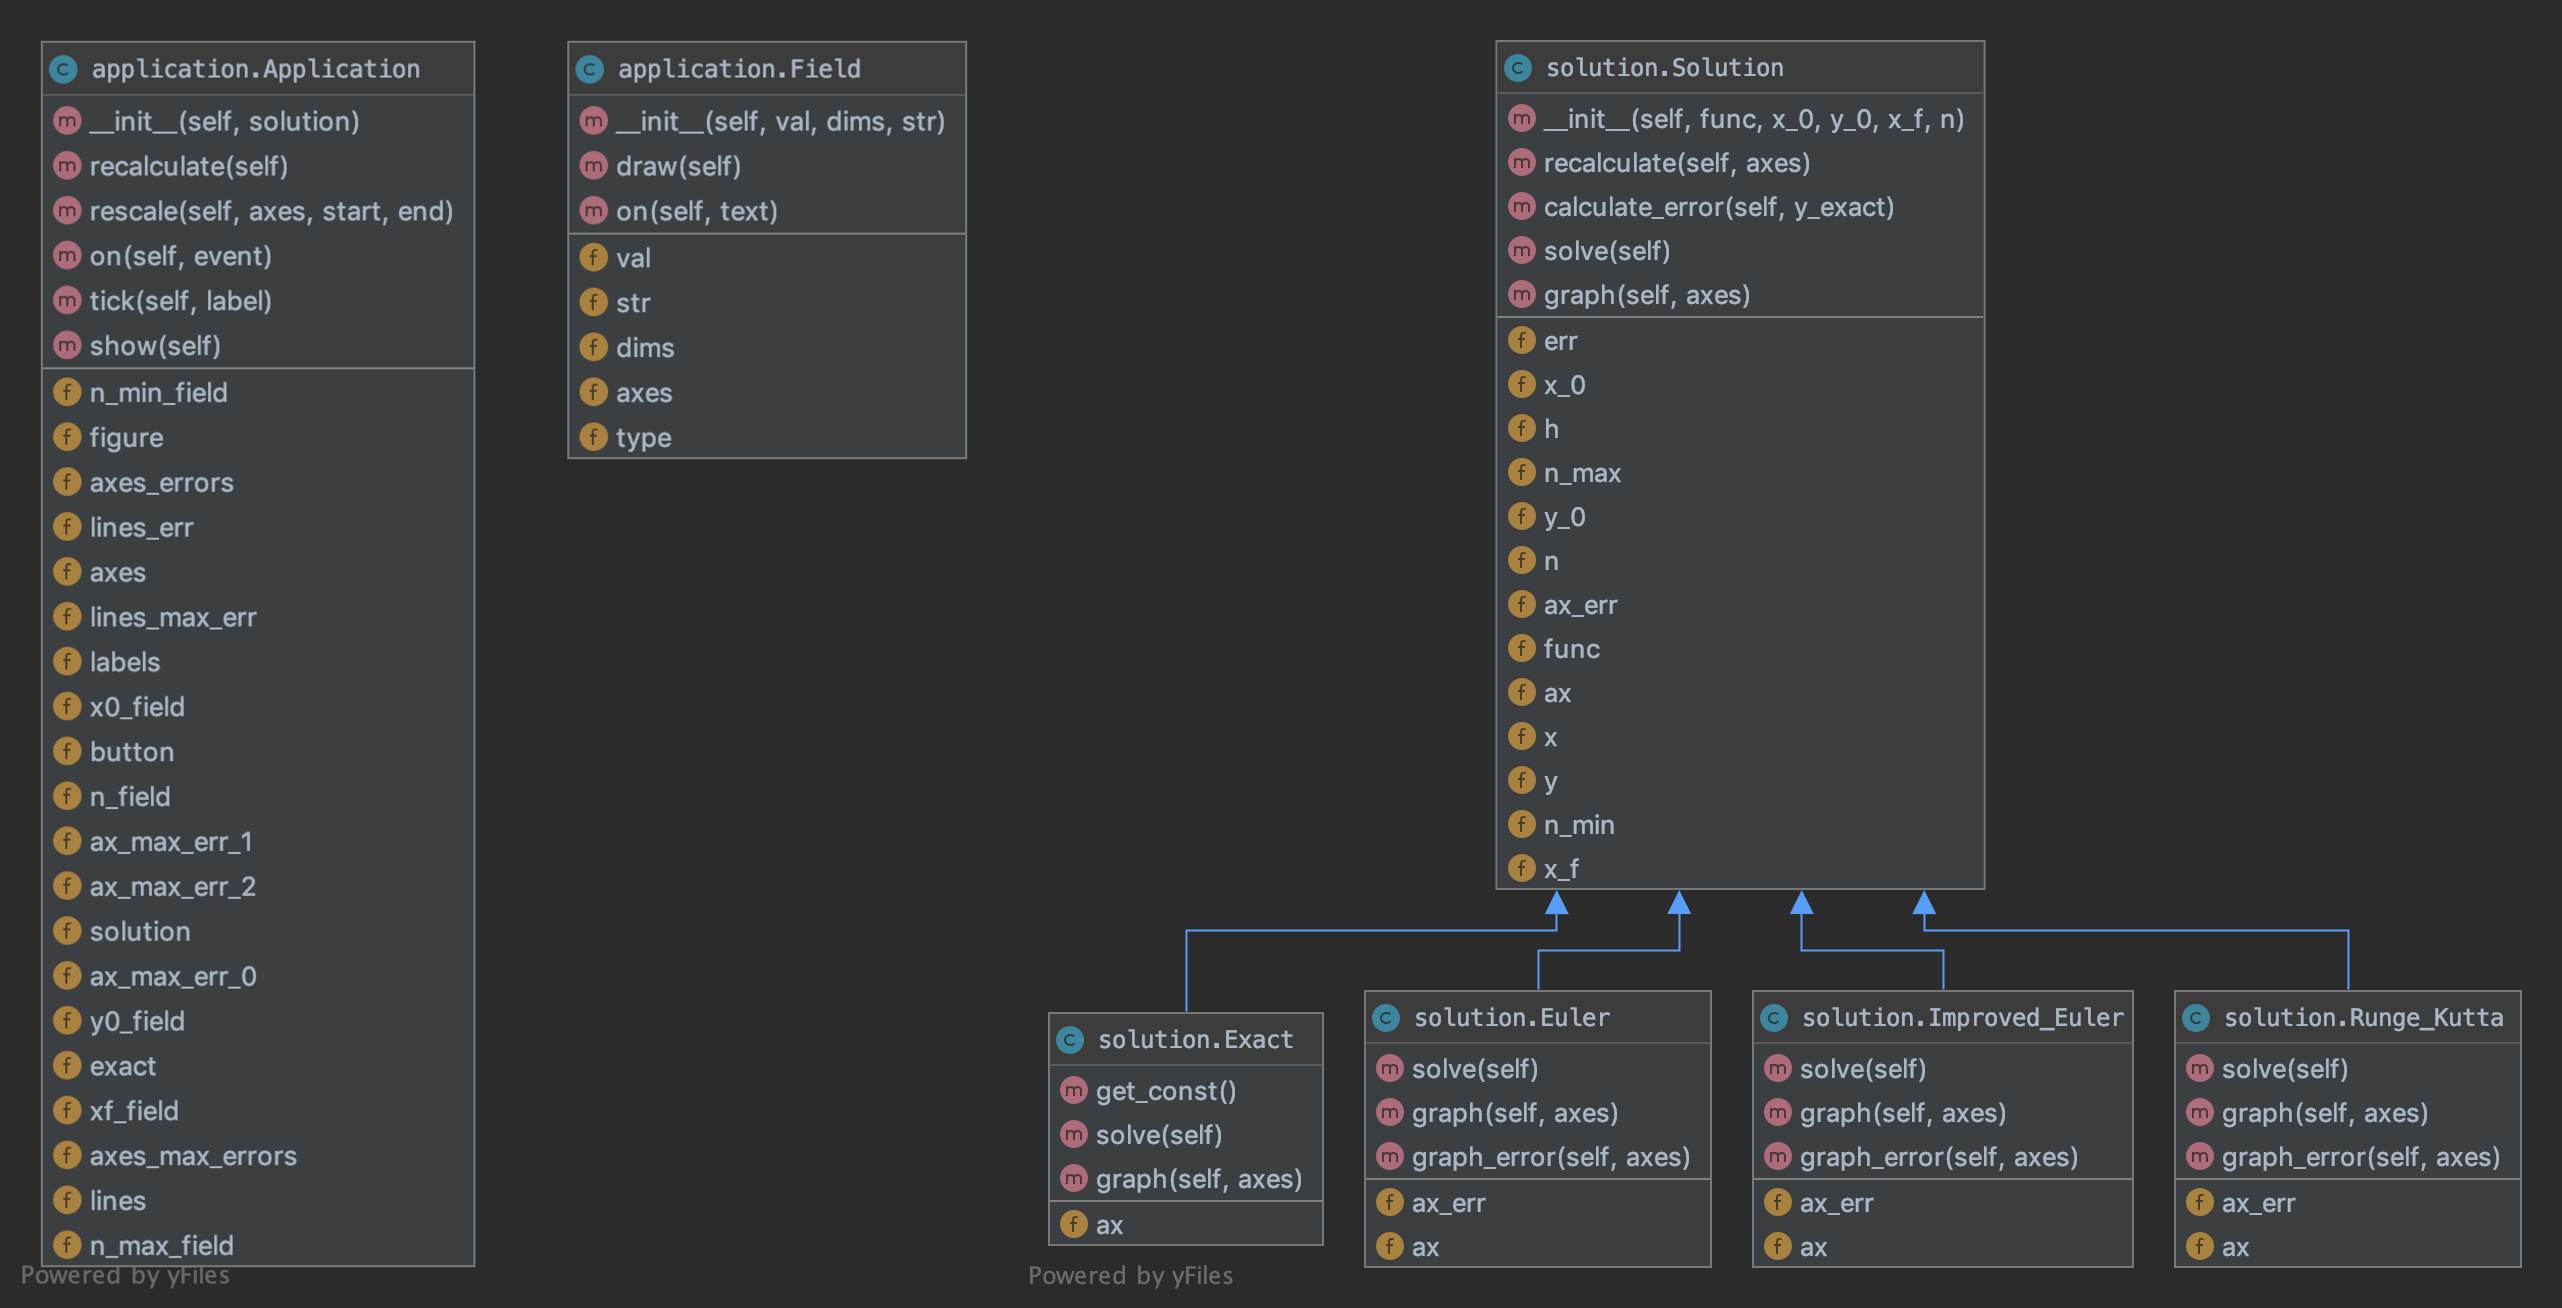
\includegraphics[width=\linewidth]{img.png}
  \caption{UML Class diagram}
  \label{fig: UML Class diagram}
\end{figure}

\paragraph{\large{Classes}}
$\\*$
There are 7 classes in my project: Application, Field, Solution, Exact, Euler, Improved Euler and Runge Kutta. If there is another function for solving IVP you need to change only 3 rows of code(solution.py: 49, 54, 103).$\\*$
\textit{Application} - class for providing GUI, an interaction between user input and computations. Also it is responsible for updating info from input fields and checkbox.$\\*$
\textit{Field} - class for textboxes that provide their initialization, drawing, and evaluation of data(their could be inserted expression, not just numbers)$\\*$
\textit{Solution} - abstract class for solutions, has the same function recalculate and calculate error for all methods.$\\*$
\textit{Exact, Euler, Improved Euler, Runge Kutta} - classes inherited from Solution. Each of them has it's own solve function, graph function and graph error(only for Exact there is no such function, because error obviously is 0.$\\*$
At the figure \ref{fig: UML Class diagram} there is UML class diagram of the project.

\newpage
\paragraph{\large{Implementation of exact solution and numerical methods}}$\\$

\textbf{Initialization} for each method:
\begin{figure}[h]
      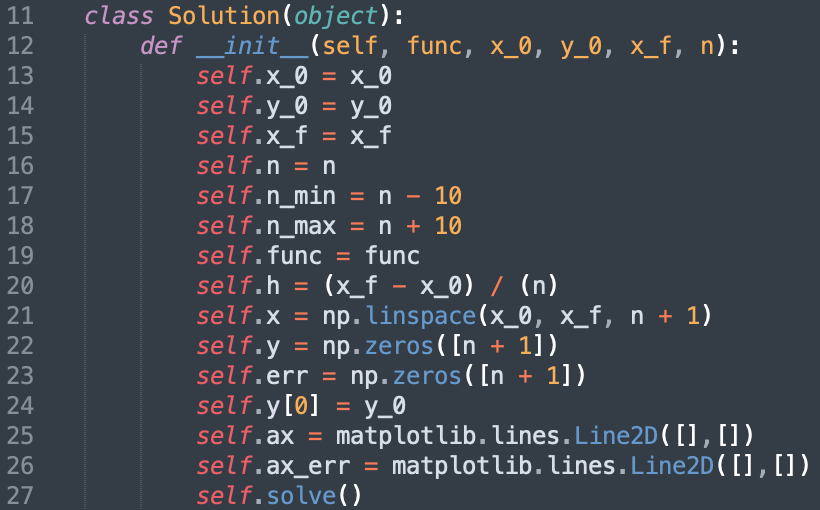
\includegraphics[width=0.65\linewidth]{init.png}
      
      \label{fig: Code}
\end{figure}

\textbf{Solve Function} for each method:
\begin{figure}[h]
    \begin{subfigure}{\linewidth}
      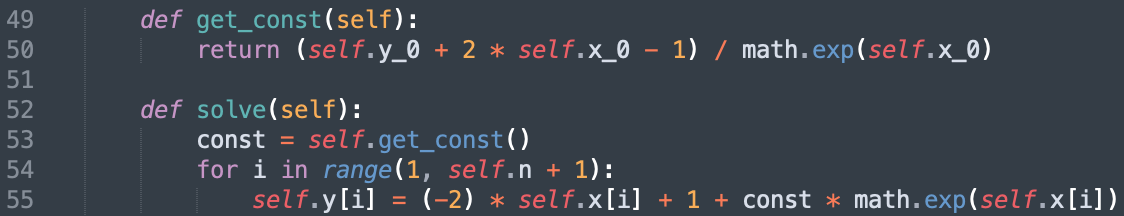
\includegraphics[width=\linewidth]{exact.png}
      \caption{Exact}
    \end{subfigure}
    \begin{subfigure}{\linewidth}
      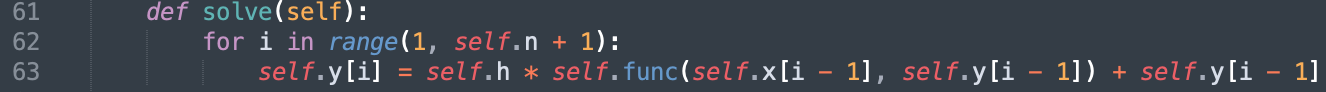
\includegraphics[width=\linewidth]{euler.png}
      \caption{Euler}
    \end{subfigure}
    \begin{subfigure}{\linewidth}
      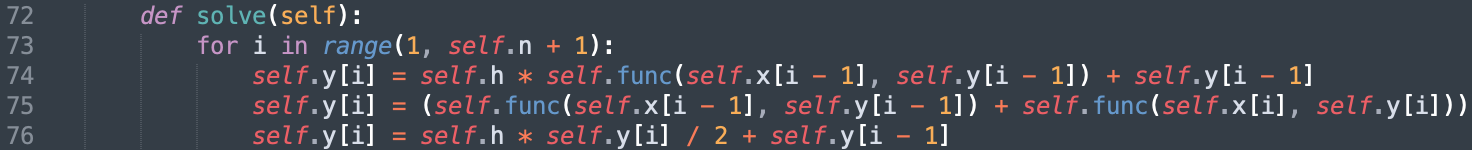
\includegraphics[width=\linewidth]{improved_euler.png}
      \caption{Improved Euler}
    \end{subfigure}
    \begin{subfigure}{\linewidth}
      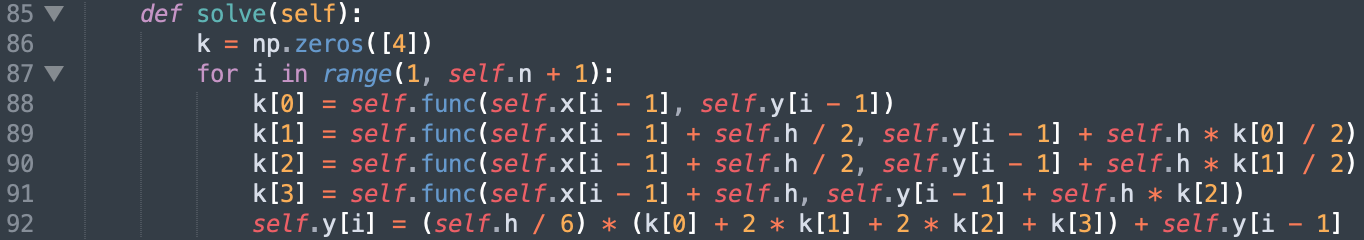
\includegraphics[width=\linewidth]{runge_kutta.png}
      \caption{Runge Kutta}
    \end{subfigure}
    \label{fig: Solve functions}
\end{figure}
\newpage

\paragraph{\large{Implementation of errors}}$\\$

\textbf{Local error} was calculated as difference between exact and approximation value of y of numerical method. This function is the same for all methods, so it was implemented in Solution abstract class.
\begin{figure}[h]
      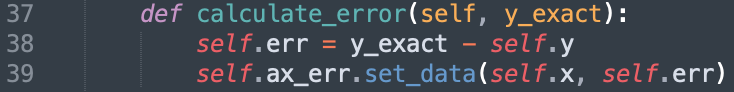
\includegraphics[width=0.8\linewidth]{local_error.png}
      \label{fig: local_error}
\end{figure}

\textbf{Total error} was calculated as maximum absolute value of local error of numerical method. These calculations were implemented in Application class.
\begin{figure}[h]
      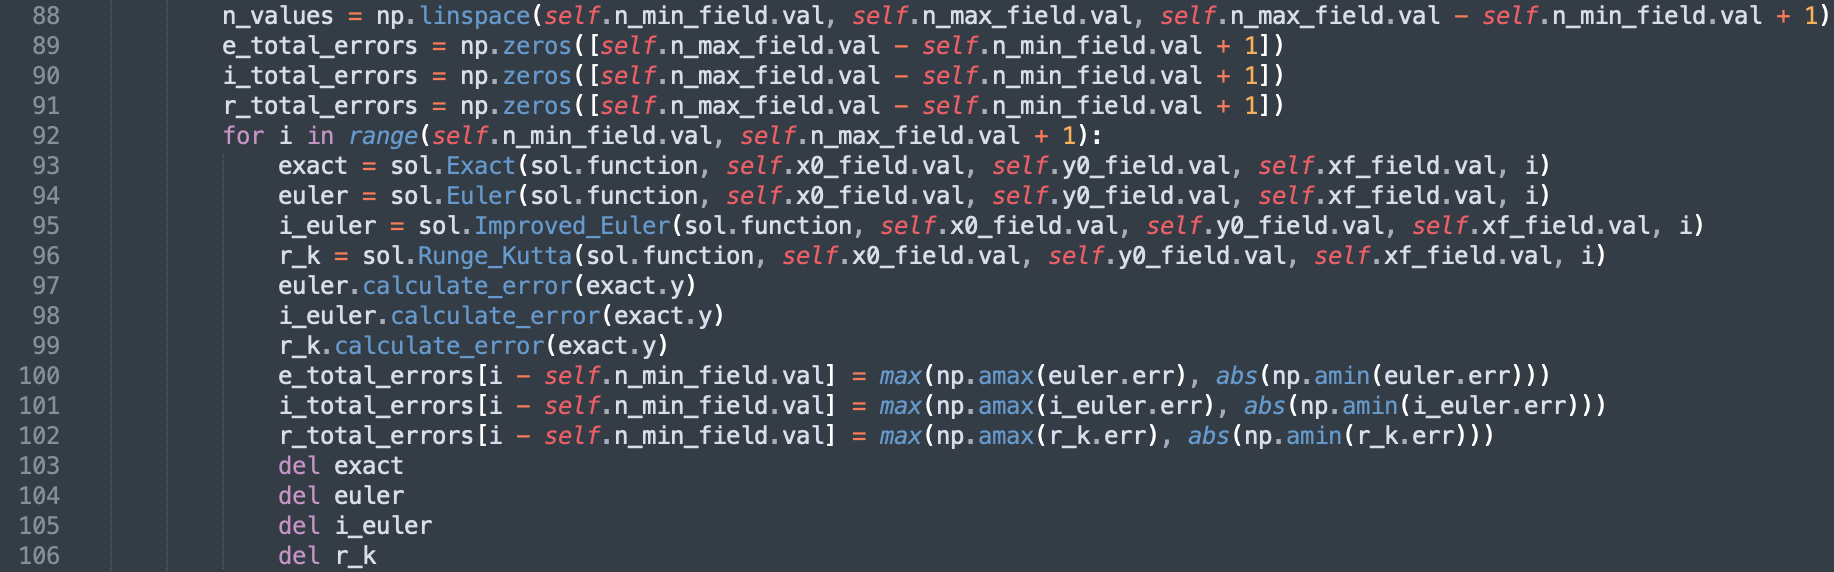
\includegraphics[width=\linewidth]{total_error.png}
      \label{fig: total_error}
\end{figure}

\section{Interface}
I used \textit{matplotlib} library for making GUI: graphs, text fields, buttons and checkboxes, for fast calculations I prefered \textit{numpy} library.

\textbf{Graphs of methods} for initial values(x0 = 1, y0 = 1, X = 7, n = 40):
\begin{figure}[h]
      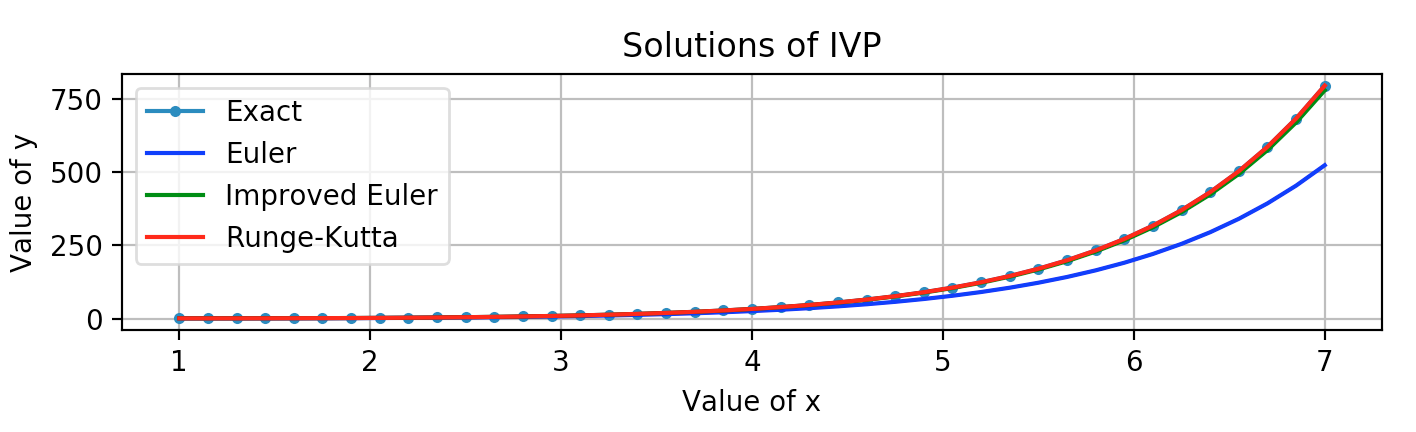
\includegraphics[width=0.8\linewidth]{exact_i.png}
      \label{fig: i1}
\end{figure}

\newpage
\textbf{Local Errors} for initial values(x0 = 1, y0 = 1, X = 7, n = 40):
\begin{figure}[h]
      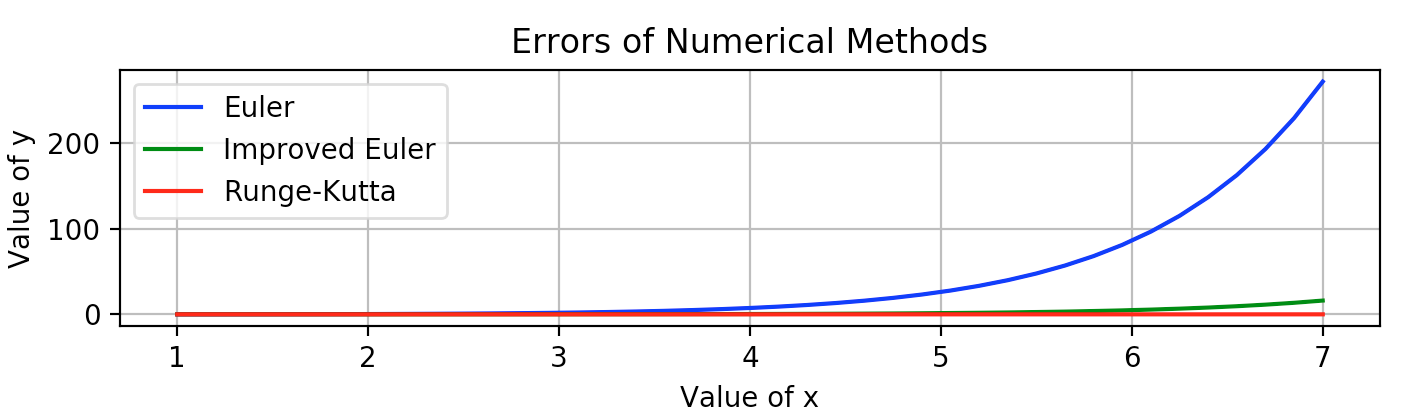
\includegraphics[width=0.8\linewidth]{local_i.png}
      \label{fig: i2}
\end{figure}

\textbf{Total Errors} for initial values(x0 = 1, y0 = 1, X = 7, nmin = 30, nmax = 50):
\begin{figure}[h]
      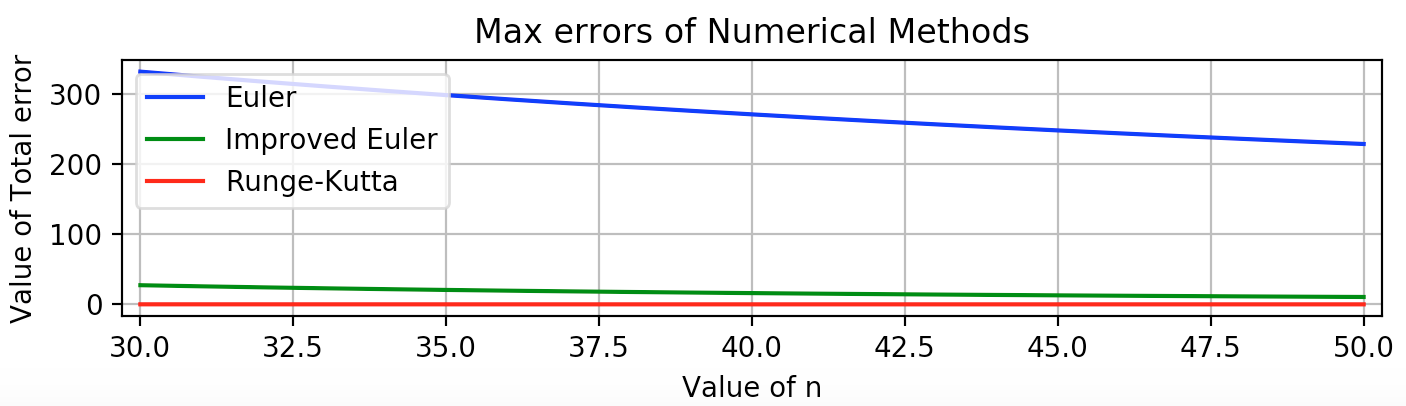
\includegraphics[width=0.8\linewidth]{total_i.png}
      \label{fig: i3}
\end{figure}

\textbf{Functionality} $\\*$
User can change initial values and by pressing button \textit{Recalculate} get new graphs for updated values. Also user can choose for which methods he/she wants to see graphs in \textit{checkbox}:
\begin{figure}[h]
    \begin{subfigure}{0.25\linewidth}
      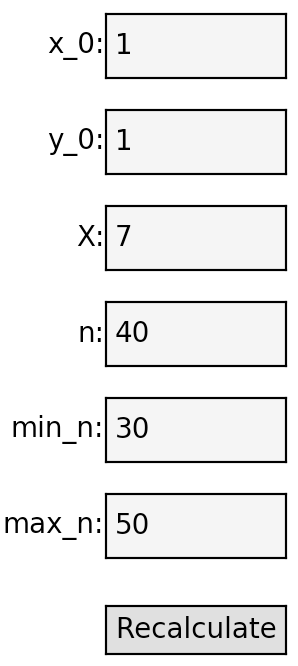
\includegraphics[width=\linewidth]{initial_values.png}
    \end{subfigure}
    \begin{subfigure}{0.3\linewidth}
      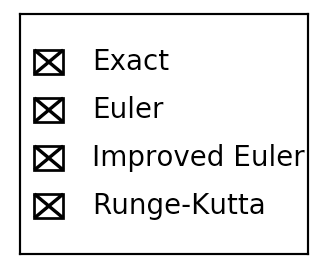
\includegraphics[width=1.5\linewidth]{checkbox.png}
    \end{subfigure}
    \label{fig: functionality}
\end{figure}
\newpage

\section{Analyses}
\paragraph{Analyses of difference of approximation in methods} 
$\\*$As we can see both from the graphs of solutions and from the errors graphs, for the given differential equation Runge-Kutta Method gives the closest approximation. This conclusion proves our theoretical computations of the approximated local error($O(h^2)$ - Euler’s method, $O(h^3)$ - Improved Euler’s Method and $O(h^5)$ - Runge-Kutta Method).

\paragraph{Analyses of difference of total errors in methods} 
$\\*$As we can guess, with less n the approximation is worse $=>$ the total error of methods is increasing, with more n the approximation is better $=>$ the total error of methods is decreasing.

\section{Source code}
You can find the implementation of the project by following the next link$\\*$ \url{https://github.com/rufusnufus/DE}
\end{document}